\subsection{Kiến trúc hệ thống}

\subsubsection{Yêu cầu kiến trúc}

Hệ thống Quản lý Co-working Space phục vụ nhiều nhóm người dùng với các vai trò khác nhau (khách hàng, nhân viên, quản lý chi nhánh, quản trị viên hệ thống), đồng thời xử lý các nghiệp vụ phức tạp và đa dạng. Để đảm bảo chất lượng và tính bền vững của phần mềm, kiến trúc hệ thống cần đáp ứng các yêu cầu phi chức năng sau:

\begin{itemize}
    \item \textbf{Khả năng mở rộng (Scalability):} Cho phép bổ sung các module nghiệp vụ mới (ví dụ: quản lý sự kiện, hệ thống điểm thưởng) mà không cần thay đổi cấu trúc tổng thể của hệ thống.
    \item \textbf{Khả năng bảo trì (Maintainability):} Các thành phần được phân tách rõ ràng theo trách nhiệm, giúp việc sửa lỗi, cập nhật và nâng cấp diễn ra độc lập, giảm thiểu rủi ro ảnh hưởng lẫn nhau.
    \item \textbf{Bảo mật (Security):} Hỗ trợ cơ chế xác thực và phân quyền đa tầng, đảm bảo mỗi vai trò người dùng chỉ truy cập được các chức năng và dữ liệu được phép.
    \item \textbf{Khả năng tích hợp (Integrability):} Dễ dàng kết nối với các dịch vụ bên thứ ba như cổng thanh toán (MoMo), dịch vụ xác thực (Google OAuth2, Supabase Authentication) thông qua các giao diện chuẩn hóa.
\end{itemize}

\subsubsection{Phân tích và lựa chọn kiến trúc}

Nhóm đã tiến hành phân tích và so sánh ba mô hình kiến trúc phổ biến trong phát triển ứng dụng web để lựa chọn phương án phù hợp nhất cho hệ thống.

\begin{table}[H]
\centering
\caption{So sánh các mô hình kiến trúc phần mềm}
\label{tab:architecture-comparison}
\renewcommand{\arraystretch}{1.4}
\begin{tabular}{|p{3.5cm}|p{3.5cm}|p{3.5cm}|p{3.5cm}|}
\hline
\textbf{Tiêu chí} & \textbf{Monolithic} & \textbf{Microservices} & \textbf{Client-Server 3-Tier + Layered} \\
\hline
Độ phức tạp triển khai & Thấp – đóng gói và triển khai dưới dạng một ứng dụng duy nhất & Cao – yêu cầu container hóa, hệ thống điều phối (orchestration) và giám sát phân tán & Trung bình – triển khai tách biệt client và server \\
\hline
Khả năng mở rộng & Hạn chế – phải mở rộng toàn bộ ứng dụng & Rất cao – mở rộng độc lập từng dịch vụ & Tốt – mở rộng theo tầng hoặc theo module nghiệp vụ \\
\hline
Khả năng bảo trì & Khó khăn khi hệ thống phát triển lớn, các module phụ thuộc chặt chẽ & Tốt – các dịch vụ độc lập, dễ cập nhật riêng lẻ & Tốt – phân tách rõ ràng theo tầng và trách nhiệm \\
\hline
Phù hợp quy mô dự án & Dự án nhỏ, đơn giản & Dự án lớn, đội ngũ nhiều người & Dự án vừa, đội ngũ nhỏ đến trung bình \\
\hline
Chi phí vận hành & Thấp & Cao – cần hạ tầng phức tạp & Trung bình \\
\hline
\end{tabular}
\end{table}

Dựa trên kết quả phân tích ở Bảng~\ref{tab:architecture-comparison}, nhóm quyết định lựa chọn mô hình \textbf{Client-Server với kiến trúc 3 tầng (3-Tier Architecture)} kết hợp \textbf{kiến trúc phân lớp (Layered Architecture)} cho phần back-end. Lý do cụ thể bao gồm:

\begin{itemize}
    \item \textbf{Cân bằng giữa tính mở rộng và độ phức tạp:} So với Monolithic, kiến trúc 3 tầng cho phép phát triển và mở rộng từng tầng một cách độc lập. So với Microservices, mô hình này có độ phức tạp vận hành thấp hơn đáng kể, phù hợp hơn với quy mô và nguồn lực của nhóm phát triển.
    \item \textbf{Phân tách trách nhiệm rõ ràng:} Kiến trúc phân lớp trong back-end (Security $\rightarrow$ Controller $\rightarrow$ Service $\rightarrow$ Repository) tuân thủ nguyên tắc \textit{Separation of Concerns}, giúp mỗi tầng chỉ đảm nhận một trách nhiệm cụ thể, từ đó tăng tính dễ đọc và bảo trì của mã nguồn.
    \item \textbf{Phù hợp với công nghệ sử dụng:} Mô hình này tương thích tốt với bộ công nghệ đã chọn — Spring Boot hỗ trợ tự nhiên kiến trúc phân lớp, React xây dựng SPA tách biệt hoàn toàn với back-end, và giao tiếp giữa hai tầng thông qua RESTful API theo chuẩn HTTP/JSON.
\end{itemize}

\subsubsection{Mô tả các thành phần kiến trúc}

\begin{figure}[H]
    \centering
    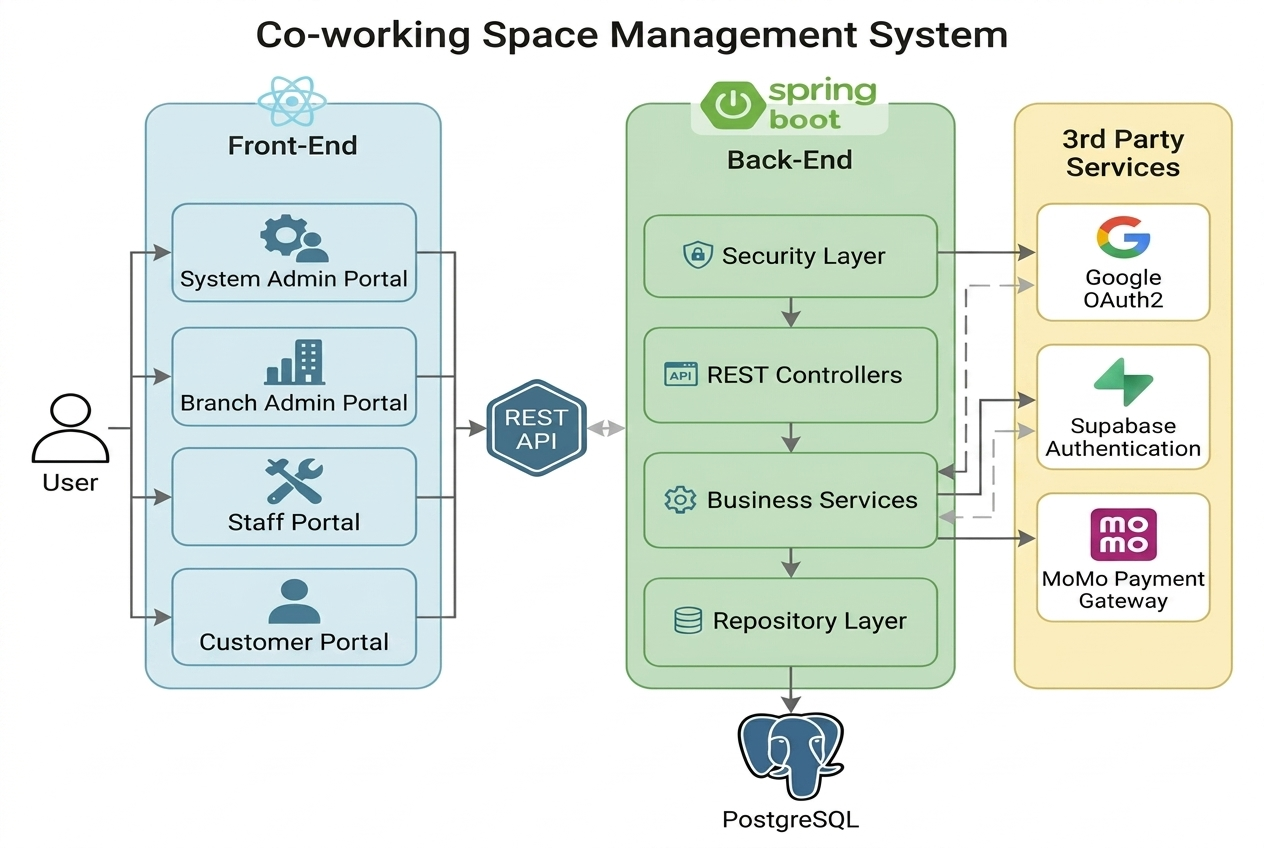
\includegraphics[width=0.85\textwidth]{Images/Chuong4/ArchitectureDiagram.png}
    \caption{Sơ đồ tổng quan kiến trúc của hệ thống}
    \label{fig:architecture-diagram}
\end{figure}

Kiến trúc của hệ thống được tổ chức thành ba tầng chính như trong Hình~\ref{fig:architecture-diagram}, cùng với các dịch vụ bên thứ ba được tích hợp. Chi tiết từng thành phần như sau:

\subsubsubsection{Tầng Trình bày (Presentation Tier)}

Tầng trình bày là một ứng dụng web đơn trang (Single Page Application -- SPA) được xây dựng bằng \textbf{React} và \textbf{TypeScript}. Giao diện được thiết kế theo hướng đáp ứng (responsive), đảm bảo trải nghiệm nhất quán trên nhiều kích thước màn hình. Ứng dụng được chia thành bốn cổng giao diện (portal), mỗi cổng phục vụ một nhóm người dùng với vai trò cụ thể:

\begin{itemize}
    \item \textbf{Customer Portal:} Cung cấp chức năng tìm kiếm không gian, đặt chỗ, thanh toán trực tuyến, xem lịch sử đặt chỗ và quản lý thông tin cá nhân cho khách hàng.
    \item \textbf{Staff Portal:} Hỗ trợ nhân viên thực hiện check-in/check-out cho khách hàng, xác nhận thanh toán, tạo đặt chỗ walk-in và quản lý vận hành hàng ngày.
    \item \textbf{Branch Admin Portal:} Cho phép quản lý chi nhánh theo dõi hiệu suất kinh doanh, quản lý không gian, nhân viên, giá cả và chính sách tại chi nhánh mình phụ trách.
    \item \textbf{System Admin Portal:} Dành cho quản trị viên hệ thống để quản lý toàn bộ chi nhánh, người dùng, chính sách giá, dịch vụ bổ sung, xem báo cáo tổng hợp và nhật ký hoạt động.
\end{itemize}

\subsubsubsection{Tầng Ứng dụng (Application Tier)}

Tầng ứng dụng được xây dựng bằng \textbf{Spring Boot (Java)} theo kiến trúc phân lớp, bao gồm bốn lớp con xếp chồng theo thứ tự xử lý yêu cầu từ trên xuống:

\begin{itemize}
    \item \textbf{Security Layer (Lớp bảo mật):} Sử dụng Spring Security để thực hiện xác thực (authentication) và phân quyền (authorization). Mọi yêu cầu HTTP đều phải đi qua lớp này trước khi được chuyển tiếp xuống các lớp bên dưới. Lớp bảo mật tích hợp với Supabase Authentication và Google OAuth2 để xác thực danh tính người dùng, đồng thời sử dụng JSON Web Token (JWT) để duy trì phiên đăng nhập và kiểm soát quyền truy cập vào các API endpoint.
    
    \item \textbf{REST Controllers (Lớp điều khiển):} Đóng vai trò là điểm tiếp nhận các yêu cầu HTTP từ tầng trình bày. Lớp này trích xuất dữ liệu từ request, chuyển tiếp đến lớp nghiệp vụ tương ứng và trả về kết quả dưới dạng HTTP Response với dữ liệu JSON. Hệ thống bao gồm các controller chính: AuthController, BookingController, PaymentController, UserController, MomoController và BranchAdminSpaceController.
    
    \item \textbf{Business Services (Lớp nghiệp vụ):} Chứa toàn bộ logic xử lý cốt lõi của hệ thống. Mỗi service đảm nhận một miền nghiệp vụ riêng biệt:
    \begin{itemize}
        \item \textit{BookingService:} Xử lý tạo, cập nhật và hủy đặt chỗ, kiểm tra xung đột lịch.
        \item \textit{PaymentService:} Quản lý luồng thanh toán và theo dõi trạng thái giao dịch.
        \item \textit{PricingService:} Tính toán giá dựa trên loại không gian, thời gian sử dụng và chính sách giá.
        \item \textit{SpaceManagementService:} Quản lý thông tin không gian, trạng thái và cấu hình.
        \item \textit{AuthService \& UserService:} Xử lý đăng ký, đăng nhập và quản lý thông tin người dùng.
        \item \textit{MomoService:} Tích hợp với cổng thanh toán MoMo để xử lý giao dịch trực tuyến.
    \end{itemize}
    
    \item \textbf{Repository Layer (Lớp truy cập dữ liệu):} Sử dụng Spring Data JPA để tương tác với cơ sở dữ liệu. Lớp này cung cấp các phương thức truy vấn dữ liệu được trừu tượng hóa, giúp lớp nghiệp vụ không phụ thuộc trực tiếp vào cú pháp SQL hay hệ quản trị cơ sở dữ liệu cụ thể.
\end{itemize}

\subsubsubsection{Tầng Dữ liệu (Data Tier)}

Hệ thống sử dụng \textbf{PostgreSQL} làm hệ quản trị cơ sở dữ liệu quan hệ. PostgreSQL được lựa chọn nhờ khả năng đảm bảo tính toàn vẹn dữ liệu với giao dịch ACID, hỗ trợ truy vấn phức tạp, kiểu dữ liệu JSON linh hoạt, và hiệu năng ổn định với lượng dữ liệu lớn. Toàn bộ dữ liệu nghiệp vụ của hệ thống -- bao gồm thông tin người dùng, đặt chỗ, thanh toán, không gian, chính sách giá -- đều được lưu trữ tại tầng này.

\subsubsubsection{Dịch vụ bên thứ ba (3rd Party Services)}

Hệ thống tích hợp với các dịch vụ bên ngoài để mở rộng chức năng mà không cần tự phát triển từ đầu:

\begin{itemize}
    \item \textbf{Supabase Authentication \& Google OAuth2:} Cung cấp giải pháp xác thực người dùng, hỗ trợ đăng nhập bằng tài khoản Google và quản lý phiên đăng nhập. Việc sử dụng dịch vụ xác thực của bên thứ ba giúp đảm bảo tính bảo mật cao và giảm thiểu rủi ro trong việc tự quản lý mật khẩu người dùng.
    \item \textbf{MoMo Payment Gateway:} Cổng thanh toán trực tuyến được tích hợp để xử lý các giao dịch thanh toán cho việc đặt chỗ, cho phép khách hàng thanh toán nhanh chóng và an toàn thông qua ví điện tử MoMo.
\end{itemize}

\subsubsubsection{Giao tiếp giữa các tầng}

Tầng trình bày và tầng ứng dụng giao tiếp thông qua \textbf{RESTful API} theo giao thức HTTP, với dữ liệu trao đổi ở định dạng JSON. Mọi tương tác từ người dùng trên giao diện đều được chuyển đổi thành các HTTP Request gửi đến các API endpoint tương ứng. Tầng ứng dụng xử lý yêu cầu và trả về HTTP Response chứa dữ liệu kết quả hoặc thông báo lỗi. Cách tiếp cận này cho phép front-end và back-end được phát triển, triển khai và mở rộng hoàn toàn độc lập với nhau.

% \end{itemize}